% Options for packages loaded elsewhere
\PassOptionsToPackage{unicode}{hyperref}
\PassOptionsToPackage{hyphens}{url}
%
\documentclass[
]{ltjarticle}
\usepackage{lmodern}
\usepackage{amssymb,amsmath}
\usepackage{ifxetex,ifluatex}
\ifnum 0\ifxetex 1\fi\ifluatex 1\fi=0 % if pdftex
  \usepackage[T1]{fontenc}
  \usepackage[utf8]{inputenc}
  \usepackage{textcomp} % provide euro and other symbols
\else % if luatex or xetex
  \usepackage{unicode-math}
  \defaultfontfeatures{Scale=MatchLowercase}
  \defaultfontfeatures[\rmfamily]{Ligatures=TeX,Scale=1}
\fi
% Use upquote if available, for straight quotes in verbatim environments
\IfFileExists{upquote.sty}{\usepackage{upquote}}{}
\IfFileExists{microtype.sty}{% use microtype if available
  \usepackage[]{microtype}
  \UseMicrotypeSet[protrusion]{basicmath} % disable protrusion for tt fonts
}{}
\makeatletter
\@ifundefined{KOMAClassName}{% if non-KOMA class
  \IfFileExists{parskip.sty}{%
    \usepackage{parskip}
  }{% else
    \setlength{\parindent}{0pt}
    \setlength{\parskip}{6pt plus 2pt minus 1pt}}
}{% if KOMA class
  \KOMAoptions{parskip=half}}
\makeatother
\usepackage{xcolor}
\IfFileExists{xurl.sty}{\usepackage{xurl}}{} % add URL line breaks if available
\IfFileExists{bookmark.sty}{\usepackage{bookmark}}{\usepackage{hyperref}}
\hypersetup{
  pdftitle={Build Back Betterにみられる育児支援策の検証},
  pdfauthor={Jake Underland (1A193008)},
  hidelinks,
  pdfcreator={LaTeX via pandoc}}
\urlstyle{same} % disable monospaced font for URLs
\usepackage[margin=2cm]{geometry}
\usepackage{graphicx,grffile}
\makeatletter
\def\maxwidth{\ifdim\Gin@nat@width>\linewidth\linewidth\else\Gin@nat@width\fi}
\def\maxheight{\ifdim\Gin@nat@height>\textheight\textheight\else\Gin@nat@height\fi}
\makeatother
% Scale images if necessary, so that they will not overflow the page
% margins by default, and it is still possible to overwrite the defaults
% using explicit options in \includegraphics[width, height, ...]{}
\setkeys{Gin}{width=\maxwidth,height=\maxheight,keepaspectratio}
% Set default figure placement to htbp
\makeatletter
\def\fps@figure{htbp}
\makeatother
\setlength{\emergencystretch}{3em} % prevent overfull lines
\providecommand{\tightlist}{%
  \setlength{\itemsep}{0pt}\setlength{\parskip}{0pt}}
\setcounter{secnumdepth}{5}
\usepackage{graphicx}
\graphicspath{ {images/} }
\usepackage{subfig}
\usepackage{amsmath}
\usepackage{color}
\usepackage{hyperref}
\usepackage{luatexja}

\title{Build Back Betterにみられる育児支援策の検証}
\author{Jake Underland (1A193008)}
\date{2022-01-17}

\begin{document}
\maketitle

\hypertarget{ux5e8fux7ae0}{%
\section{序章}\label{ux5e8fux7ae0}}

~~~~教育経済学の研究が進み,早期幼児教育の好影響が明らかになっている中(Heckman
et al.,
2020),アメリカ合衆国では手の届く価格での高クオリティな保育所やチャイルドケアを求める声が高まっている.\\
\hspace*{0.333em}\hspace*{0.333em}\hspace*{0.333em}\hspace*{0.333em}一方で,アメリカ国内の保育所を見ると,クオリティの高いものはあまりにも高価で多くの家庭の手が届かず,一般の家庭の手が届く範囲のものはクオリティが低いという批判を長く受けてきた(NICHD,
1998; First Five Years Fund, 2021).\\
\hspace*{0.333em}\hspace*{0.333em}\hspace*{0.333em}\hspace*{0.333em}こうした声に応え,コロナ対策案として施行されたAmerican
Rescue Planでは,米国の育児支援給付金であるChild Tax
Creditが一時的に拡大され,バイデン政権下で拡大の期限が延長されるなど,チャイルドケアへの公的投資が増えてきている.この流れに沿い,現時点で法案が下院議会を通過し,上院で予算が協議されているインフラ投資政策Build
Back Betterでも,早期幼児教育への多額な出資が含まれている.特にBuild
Back
Betterのなかの育児支援政策では,政府はチャイルドケアへの投資を通じて全ての子育て世帯に手頃な価格で高いクオリティの保育所,託児所等へのアクセスを保障したい意図が見える.意図自体は褒むべきものであるが,支援案の詳細がその意図の実現に適切であるかどうかを本レポートで検討していく.

\hypertarget{ux653fux7b56ux6982ux8981}{%
\section{政策概要}\label{ux653fux7b56ux6982ux8981}}

~~~~Build Back Better
に含まれる育児支援政策は,およそ2部構成となっている.一つは,6歳以下の子持ち世帯への条件づき金銭援助であり,もう一つは,州政府が保育所の増設,改良といった幼児教育投資をするための予算援助である.\\
\hspace*{0.333em}\hspace*{0.333em}\hspace*{0.333em}\hspace*{0.333em}各家庭への金銭的援助では,様々な条件に応じて援助額を調整する.まず,州ごとの物価の違いを考慮し,支援額を決定する基準となる所得水準は州ごとの中央値を使う.施行から3年後にはフェーズインが終了し,所得が各州の所得分布の中央値の250\%以下で少なくとも一方の親が労働,求職,研修等で労働市場に参画している家庭が給付の対象となる.金銭給付額は所得に応じて変動するが,6歳以下の子供の人数に合わせた補助金が給付され,また給付条件に該当する全ての家庭のそれぞれの子育て費用が最大でもその家庭の所得の7\%以下となることを保障する.\\
\hspace*{0.333em}\hspace*{0.333em}\hspace*{0.333em}\hspace*{0.333em}多くの給付条件が存在するものの,総じて6歳以下子持ち世帯のうち約9割の世帯が援助の対象となる.また,The
Center for American Progress
(2021)の試算では,一般的な6歳以下子持ち世帯(所得がSMIの135\%)が受ける援助額は,全州を平均して約\(\$120\)である.援助は保育園の学費を主とする子持ち世帯の子育て費用に紐づけられており,税控除という形をとるので,自由に使い道を決定できる現金給付とは異なる点は留意すべきである.\\
\hspace*{0.333em}\hspace*{0.333em}\hspace*{0.333em}\hspace*{0.333em}州政府への援助は,州が新たな保育所を建設し,既存の保育所の改修を行えるようにする.予算の具体的な運用方法は州政府の判断に委ねられるが,そこには州が運営する公立の保育所への投資も含まれれば,私的保育所への投資も含まれている.また,投資を受ける保育所ではそこで働く保育士の給料が見直され,連邦政府が定めたガイドラインのもと,仕事に見合う賃金が払われることが求められる.保育所のクオリティも段階方式で評価され,投資を受ける保育所は一定のクオリティを上回ることが条件とされる.\\
\hspace*{0.333em}\hspace*{0.333em}\hspace*{0.333em}\hspace*{0.333em}以上をまとめると,本政策の根幹を成すのは,保育サービスを需要する家庭,供給する事業者の双方への補助金である.

\hypertarget{ux653fux7b56ux76eeux7684}{%
\section{政策目的}\label{ux653fux7b56ux76eeux7684}}

~~~~これらの政策の目的は,6歳以下の全ての子供に高いクオリティの幼児教育をもたらすことである.まず,家庭に直接援助を行うことで経済的な事情から保育所に子供を入れられない家庭を減らし,また州政府への予算援助によって新たな保育所の設置,既存の保育所の拡大を行うことで保育所や保育サービス自体の供給を整えることが政策の主眼である.\\
\hspace*{0.333em}\hspace*{0.333em}\hspace*{0.333em}\hspace*{0.333em}この政策では,州政府への予算援助の部分が効率性の達成という目標に向けた取り組みである.この市場での効率的な結果とは,全ての子育て家庭がそれぞれ望むクオリティの保育所に子供を預けられることだ.しかし,現在アメリカでは保育所の数が足りておらず(First
Five Years Fund,
2021),序章でも述べた通り,既存の保育所のクオリティは悪い.つまり,需要に供給が見合わず,子供を保育所に預けたいのに預けられない家庭が生じている.保育所を増設し,既存の保育所のクオリティをあげることを通し,政府は保育市場での過少供給を解消しようとしていると解釈できる.\\
\hspace*{0.333em}\hspace*{0.333em}\hspace*{0.333em}\hspace*{0.333em}次に,政府は支援を所得と紐づけることにより,公平性を保とうとしている.支援の対象を全ての家庭に拡げず,生活に困窮している家庭から支援を行っていく姿勢は,弱者への再分配を意識したものである.また,支援を育児・保育関連の費用に限定しているのも,本当に「保育」という財を必要としている,あるいは強く望んでいる家庭を支援しようという公平性への配慮から来るものだと考えられる.

\hypertarget{ux59a5ux5f53ux6027ux306eux691cux8a3c}{%
\section{妥当性の検証}\label{ux59a5ux5f53ux6027ux306eux691cux8a3c}}

~~~~政策概要の章でまとめた通り,本政策はその本質では保育市場に参加する消費者と生産者(公私含む保育サービスを提供する事業者)への補助金として理解することができる.この補助金の妥当性を検証するにあたり,注意しなければならないアメリカの保育市場の特徴が2点ある.それは,保育というサービスが正の外部性をもたらすということと,ある価格帯の保育市場では生産者と消費者の間に情報の非対称性が存在していることである.

\hypertarget{ux5916ux90e8ux6027}{%
\subsection{外部性}\label{ux5916ux90e8ux6027}}

~~~~社会経済的地位が高くない家庭の子育てへの早期介入(小学校入学前の保育サービス)は,子供の将来の収入,健康,その他の指標に正の効果をもたらすことが観察されている.Heckmanら
の研究者チームは早期教育への投資の社会的リターンは実に16\%にのぼると主張している(2020).早期教育により実現するこれら正の効果は,家庭自体は感じにくいだろう(保育を求める家庭にとって,子供の遠い未来の収入や健康の不確実で狭い範囲での変動がその保育サービスの便益として受け取られにくいことは想像に難くない).しかし,社会全体にとっては,健康で高スキルな労働人口が増えることはれっきとした便益として映る.図1のGraph
Aでは,こうした事実を踏まえ,私的限界便益と社会的限界便益を区別して書いている.この時,二つに差異があると,社会的限界便益が社会的限界費用を上回るにも関わらず取引がされない死荷重の領域が発生する.\\
\hspace*{0.333em}\hspace*{0.333em}\hspace*{0.333em}\hspace*{0.333em}Graph
Bは,Build Back Better
の内容となる消費者,生産者への補助金を反映させたものである.消費者への補助金は私的限界便益曲線を上方へ平行移動させ,生産者への補助金は私的限界費用曲線を下方へ平行移動させる.補助金は社会的な便益を私的便益,私的費用へと組み込むことで,外部性を私的市場に内在化している.グラフで示されている通り,理論的にはこうした双方への補助金によって社会的な最適解と等しい総余剰をもたらす均衡点にたどり着くことができる.ただし,それは補助金が従量的に課された場合である.実際,家庭への補助金額は6歳以下の子供の人数に依り,保育を供給する事業者についても,保育園単位で補助金を受ける.よって,いずれの補助金も従量的であると解釈することができる.補助金の量については計量的な問題なので何も言えないが,補助金という政策の方向自体は外部性に関する取り組みとしては適切である.

\begin{figure}
\caption{保育市場の外部性}
\centering
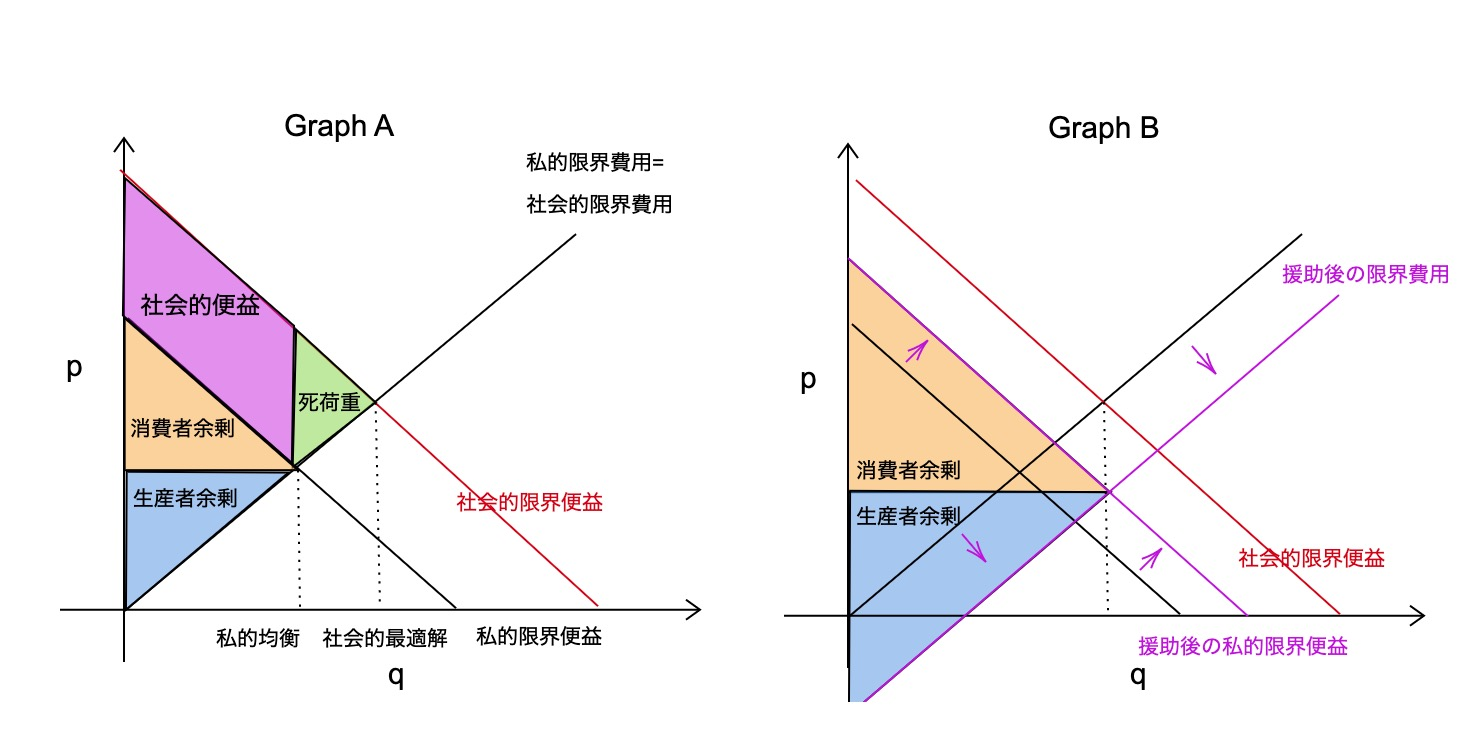
\includegraphics[width=\textwidth]{fig1.jpg}
\end{figure}

\hypertarget{ux60c5ux5831ux306eux975eux5bfeux79f0ux6027}{%
\subsection{情報の非対称性}\label{ux60c5ux5831ux306eux975eux5bfeux79f0ux6027}}

~~~~上の議論は,保育市場が競争的な市場として機能していることを前提としている.しかし,実際はある価格帯の保育園市場には情報の対称性がなく,逆選択が起こっている可能性が高い.\\
\hspace*{0.333em}\hspace*{0.333em}\hspace*{0.333em}\hspace*{0.333em}保育所や保育サービスという財は,購入する親が自ら受けることはない財である.保育所に預かられて内部まで見ることができるのは6歳以下の子供であり,子供が適切に保育園の質を評価して親に伝達するとは期待できないので,親は外から内部のクオリティを推量して保育所を選ぶほかない.その選択過程に多大な時間をかけることができるならまだしも,社会経済的地位(SES)が低い家庭は共働きあるいは働いているシングルペアレントが多く,思うほど時間をかけられない.加えて,文化資本や認知機能の低さ,アメリカではマイノリティの方だと言語バリアもある.こうした要因が重なった結果,低SES家庭の親は保育所の質を十分に審査する力がないと考えられる.保育所の質が高いものと低いものとの見分けがつかない場合,家庭は市場に出回っているサービスから受けられる便益の期待値しか払わない.その結果,高い質の保育所を提供する事業者が十分に需要を確保することができずに市場から退出し,低い質の保育所だけが残る.これが逆選択であり,アメリカの保育所不足と既存の保育所の質の低さは逆選択の結果として説明できる(Mocan,
2001).\\
\hspace*{0.333em}\hspace*{0.333em}\hspace*{0.333em}\hspace*{0.333em}他方で,SESの高い家庭では,片親が働かずに育児に集中しているか,働いていたとしても仕事のスケジュールが柔軟で時間的な余裕があると考えられる.さらに,認知能力,文化資本の量も比較的高いことが予想される.すると,これらの家庭の親は保育サービスの質を高い精度で推量することが可能となり,情報の非対称性はなく市場が機能する.アメリカで高価で高い質の保育所は多くあり,安価でそこそこの質の保育所のように市場で決定的に不足している現実が確認できないのは,こちらの高い質の保育所の市場が機能している証拠である.\\
\hspace*{0.333em}\hspace*{0.333em}\hspace*{0.333em}\hspace*{0.333em}低\textasciitilde 中価格帯の情報の非対称性問題は政府が解消するべきである.ここでは供給者が財の価値に関する情報を有し,消費者がそれを観察できないことで問題が生じているので,政府にできることは供給者の質を消費者に正確にシグナリングすることである.例えば,政府が保育所の監査機関を設置し,この機関が保育所を調査し,その実態を多層的な評価基準で評価して一般に公開することである.実際,本政策の主眼ではないが,政府は援助をする保育所の運営を評価し,一定水準以上の質を提供するように質を規制することを掲げている.質を規制することは安価で低クオリティの保育所を駆逐する実質的な価格統制であり,その価格帯の保育所を需要する家庭もそれを入手できなくなってしまうので,非効率性が生じる.規制はせず,政府は保育所の質を調査し,公開することに徹するべきである.そうすれば,市場の機能が回復し,政府の介入なくして効率的な取引が市場で行われるようになる.\\

\begin{figure}%
    \centering
    \subfloat[\centering 保育市場]{{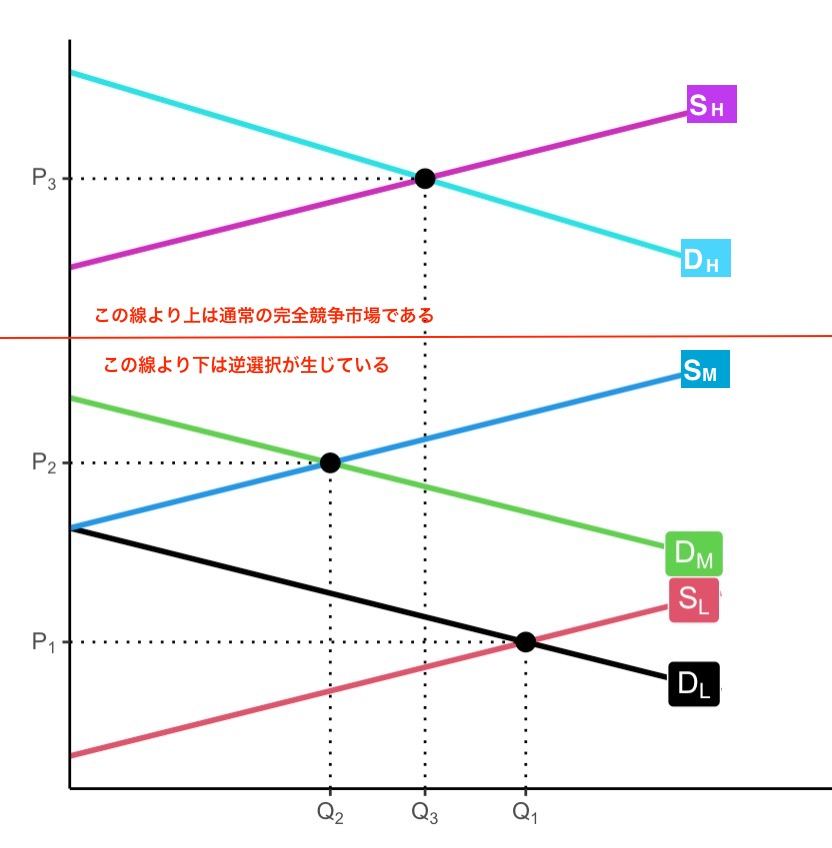
\includegraphics[width=7cm, height=7cm]{childcaremarket.jpg} }}%
    \qquad
    \subfloat[\centering 低〜中品質での逆選択の過程]{{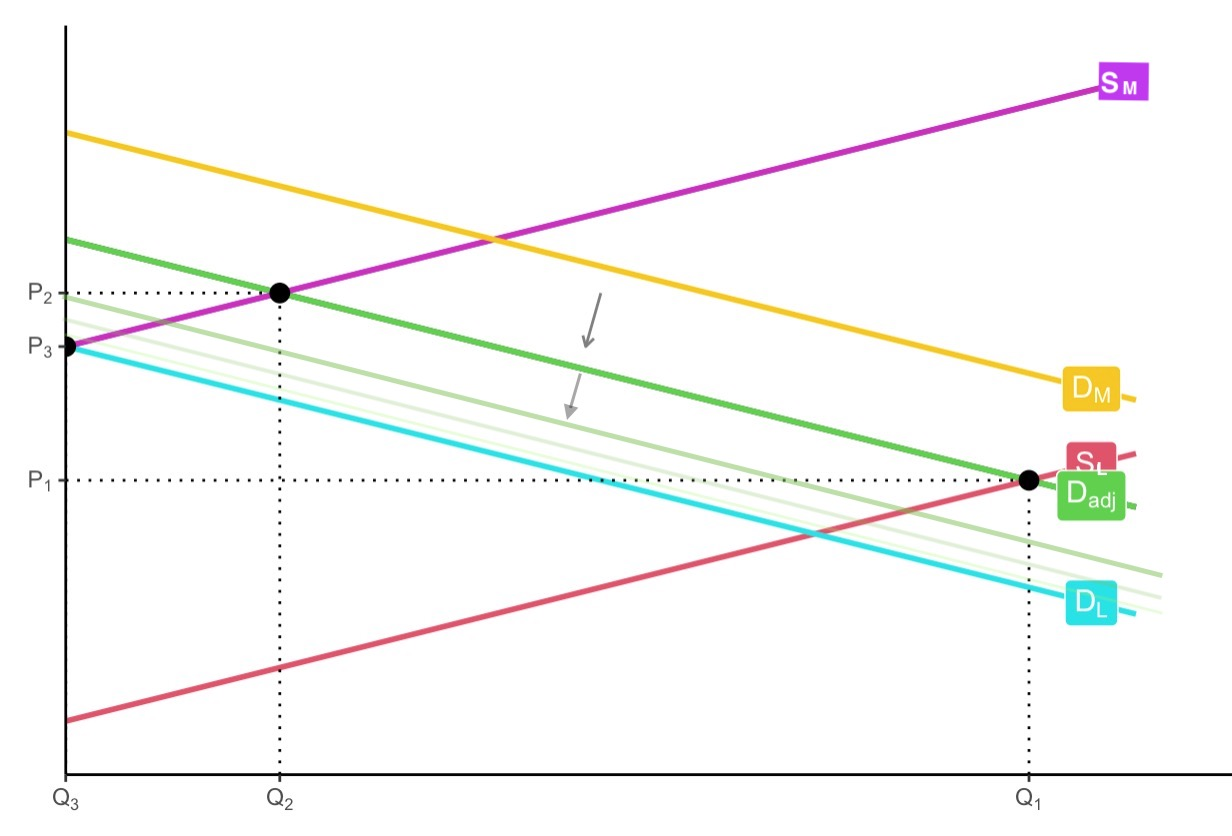
\includegraphics[width=7cm, height=7cm]{adverseselection.jpg} }}%
    \caption{(a)は保育市場に並立する高品質,中品質,低品質(H, M, L) の保育所に対応する需給曲線を書いたものである.(b)は,そのなかでも消費者に区別がつかないM, Lの保育所に注目している.(a)の市場でそれぞれが均衡に落ち着くと,市場にあるL,Mの比$L:M$に相当する$\frac{Q_1}{Q_2}$が大きい.よって,消費者は低品質の保育所と契約してしまう可能性を考慮し,需要を$D_{adj}$に調整する.すると,$\frac{Q_1}{Q_2}$はさらに大きくなり,それに応じて消費者も需要曲線を調整し,最終的に$D_{adj}$は$D_L$に収束する.すると,中品質の保育所は供給されなくなる.}
    \label{fig:example}%
\end{figure}
\newpage

\hypertarget{ux7d50ux8ad6}{%
\section{結論}\label{ux7d50ux8ad6}}

~~~~前章の議論をまとめると,アメリカ政府はまず保育市場における情報の対称性を確保し,その後に外部性の是正となる補助金を配給するべきである.情報の非対称性を残したまま金銭的補助をしようが,また逆選択が発生するだけだ.情報の非対称性を解消するだけでも過少供給はかなり緩和されることが予想されるため,それから補助金の額を定めるのが賢明だ.\\
\hspace*{0.333em}\hspace*{0.333em}\hspace*{0.333em}\hspace*{0.333em}最後に,本政策の公平性への取り組みにも触れたい.補助金を所得の高くない家庭に給付する良し悪しは規範的な問題であり,社会の価値観による.他方,補助金を特定の財と結び付けてしまうのは,特定の財の取引量を均衡から歪めてしまう.今回の場合,保育の市場には外部性が存在しているため,財に紐付けた給付金はこの外部性を市場に内在化し,社会的に最適な取引量へ調節する働きを持っている.そのため,財に紐づけた補助金は適切である.ただし,これは弱者の救済という政府の掲げる公平性への目標に合目的的であるからではなく,あくまで効率性を確保する手段であることは特記すべきだ.実のところ,本政策には公平性の確保という目的はあまり重要でないのかもしれない.

\hypertarget{references}{%
\section{References}\label{references}}

\setlength{\parindent}{-0.2in}
\setlength{\leftskip}{0.2in}
\setlength{\parskip}{8pt}

\noindent

García, J. L., Heckman, J. J., Leaf, D. E., \& Prados, M. J. (2020).
Quantifying the life-cycle benefits of an influential early-childhood
program. Journal of Political Economy, 128(7), 2502-2541.

Guarino, A. (2021). \emph{FAQ on the Child Care and Preschool Provisions
in the Build Back Better Act}. First Five Years Fund.
\url{https://www.ffyf.org/faq-on-the-child-care-and-preschool-provisions-in-the-build-back-better-act/}

Malik, R. (2021). \emph{The Build Back Better Act Would Greatly Lower
Families' Child Care Costs}. The Center for American Progress.
\url{https://www.americanprogress.org/article/build-back-better-act-greatly-lower-families-child-care-costs/}

Mocan, N. H. (2001). \emph{Can consumers detect lemons? Information
asymmetry in the market for child care} (NBER Working Paper No.~8291).
National Bureau of Economic Research.
\url{https://www.nber.org/papers/w8291}

\end{document}
